\documentclass[10pt,a4paper,twoside]{article}

%\usepackage[T1]{fontenc} % for at f� �,�, � og bogstaver med accenter 
\usepackage[latin1]{inputenc} % definer formatet p� din tekst fil 
\usepackage{lmodern} % vektor-font og flottere accenter
%\usepackage[danish]{babel} % dansk orddeling og autotekst

%\usepackage{amsmath} %several new commands that are more powerful and flexible than the ones provided by plain LaTeX

%\usepackage{a4wide}

%Check wether compiling is done under latex or pdflatex
\ifx\pdftexversion\undefined
	\usepackage[dvips]{graphicx}
\else
	\usepackage[pdftex]{graphicx}
\fi
%\usepackage{epstopdf}
\graphicspath{{./graphics/}}

\usepackage[small,bf]{caption} % Tekststil p� caption-tekst i figurer

\usepackage[colorlinks=true]{hyperref} % URL formatering
%\hypersetup{pdfborder = {0 0 0 0}} % Ingen rammer omkring URLs

%\setlength{\parskip}{5mm plus3mm minus2mm} % The spacing between paragraphs
%\setlength{\parindent}{5mm} % Indryk i nye afsnit

\usepackage[round]{natbib}

\usepackage{mparhack} %Marginpar's occur on the correct side

\usepackage{tabularx} %Tables that stretch to fit page width

\usepackage{siunitx}

\usepackage{listings} %Syntax highlighting
\usepackage{color}      % use if color is used in text
\usepackage{textcomp}
\definecolor{listinggray}{gray}{0.9}
\definecolor{lbcolor}{rgb}{0.9,0.9,0.9}
\lstset{
	%backgroundcolor=\color{lbcolor},
	tabsize=4,
	rulecolor=,
	language=MATLAB,
        basicstyle=\small,
        upquote=true,
        aboveskip={0.5\baselineskip}, 
        belowskip={1.5\baselineskip}, 
        columns=fixed,
        showstringspaces=false,
        extendedchars=true,
        breaklines=true,
        prebreak = \raisebox{0ex}[0ex][0ex]{\ensuremath{\hookleftarrow}},
        %frame=single, 
        showtabs=false,
        showspaces=false,
        showstringspaces=false,
        identifierstyle=\ttfamily,
        keywordstyle=\color[rgb]{0,0,1},
        commentstyle=\color[rgb]{0.133,0.545,0.133},
        stringstyle=\color[rgb]{0.627,0.126,0.941},
        %numbers=left, %Line numbers: left, right, none
}

%Flow chart package
\usepackage{tikz}
\usetikzlibrary{shapes,arrows}
% Define block styles
\tikzstyle{processor} = [diamond, draw, %fill=blue!20, 
    text width=4.5em, text badly centered, node distance=3cm, inner sep=0pt]
\tikzstyle{harddrive} = [rectangle, draw, fill=black!15, 
    text width=7em, text centered, rounded corners,node distance=2.5cm, minimum height=4em]
\tikzstyle{mem} = [rectangle, draw, %fill=blue!20, 
    text width=5.5em, text centered, rounded corners,node distance=2.5cm, minimum height=4em]
%\tikzstyle{line} = [draw, -latex']
\tikzstyle{cloud} = [draw, ellipse, %fill=red!20, 
					node distance=3cm, minimum height=1em]


\usepackage{fancyhdr}
\setlength{\headheight}{15.2pt}
\pagestyle{fancy}
\lhead{\fancyplain{}{\texttt{SPHERE} documentation}}
%\addto\captionsenglish{\renewcommand*\abstractname{About these notes}}

\begin{document}
\title{Users guide to \texttt{SPHERE}:\\ GPU based discrete element method software}
\author{Anders Damsgaard Christensen\\
	\url{anders.damsgaard@geo.au.dk}\\
	\url{http://cs.au.dk/~adc/}}
	\date{Last revision: \today \\[5mm] Version \textbf{0.1} \\ 
	%\begin{center} \includegraphics[scale=0.12]{FigCover} \end{center}
	}
\maketitle

\thispagestyle{empty}

\begin{abstract}
\noindent This document is the official documentation for the \texttt{SPHERE} discrete element modelling software. It presents the theory behind the discrete element method (DEM), the structure of the software \texttt{C} source code, and the {\sc Matlab} configuration methods for handling input- and output data. 

\texttt{SPHERE} is developed by Anders Damsgaard Christensen under supervision of David Lundbek Egholm and Jan A. Piotrowski, all of the department of Geology, University of Aarhus, Denmark. This document is a work in progress, and is still in an early, unfinished state. This document is typeset with \LaTeXe, with a wide margin (\LaTeX{} standard) to make space for handwritten notes.
\end{abstract}
\vfill

\begin{figure}[htb]
 \begin{center}
	\includegraphics[width=0.9\textwidth]{quiver3.eps}
 \end{center}
\end{figure}

\newpage

\section*{Revision history}
\begin{table}[htb]
  \centering 
  \begin{tabularx}{1.0\textwidth}{l c c X}
\textbf{Date} & \textbf{Doc. version} & \textbf{\texttt{SPHERE} version} & \textbf{Description} \\
\hline
2010-12-06  & 0.1 & Beta 0.03  & Initial draft \\
%   &  &  \\
%   &  &  \\
\hline
\end{tabularx}
%  \caption{ }
  \label{tab:Changelog}
\end{table}

\newpage

\newpage
\tableofcontents
\newpage

\section{Introduction}
The \texttt{SPHERE}-software is used for three-dimensional discrete element method (DEM) particle simulations. The source code is written in \texttt{C}, and compiled by the user. The main computations are performed on the graphics processing unit (GPU) using NVIDIA's general purpose parallel computing architecture, CUDA. 

The ultimate aim of the \texttt{SPHERE} software is to simulate soft-bedded subglacial conditions, while retaining the flexibility to perform simulations of granular material in other environments. The requirements to the host computer are:
\begin{itemize}
  \item UNIX, Linux or Mac OS X operating system.
  \item GCC, the GNU compiler collection.
  \item A CUDA-enabled GPU with compute capability 1.1 or greater\footnote{See \url{http://www.nvidia.com/object/cuda_gpus.html} for an official list of NVIDIA CUDA GPUs.}.
  \item The CUDA Developer Drivers and the CUDA Toolkit\footnote{Obtainable free of charge from \url{http://developer.nvidia.com/object/cuda_3_2_downloads.html}}.
\end{itemize}
For simulation setup and data handling, a {\sc Matlab} installation of a recent version is essential. There is however no requirement of {\sc Matlab} on the computer running the \texttt{SPHERE} calculations, i.e. model setup and data analysis can be performed on a separate device. Command examples in this document starting with the symbol '\verb"$"' are executed in the terminal of the operational system, and '\verb">>"' means execution in {\sc Matlab}. All numerical values in this document, the source code, and the configuration files are typeset with strict respect to the SI unit system.

\section{Discrete element method theory}
\label{sec:DEMtheory}
The discrete element method (or distinct element method) was initially formulated by \citet{Cundall:1979}. It simulates the physical behavior and interaction of discrete, unbreakable particles, with their own mass and inertia, under the influence of e.g. gravity and boundary conditions such as moving walls. By discretizing time into small time steps ($\Delta t \approx 10^{-8} \si{\second}$) eulerian integration of Newton's second law of motion is used to predict the new position and kinematic values for each particle from the previous sums of forces. This lagrangian approach is ideal for simulating discontinuous materials, such as granularities. The complexity of the computations is kept low by representing the particles as spheres, which keeps contact-searching algorithms simple.


\section{\texttt{SPHERE} source code structure}
\label{sec:spheresrcstructure}
The source code is located in the \texttt{sphere/src/} folder, and named \texttt{sphere.cu}. After compiling the \texttt{SPHERE} binary (see sub-section \ref{subsec:compilation}), the procedure of a creating and handling a simulation is typically arranged in the following order:
\begin{enumerate}
	\item Setup of particle assemblage, physical properties and conditions in {\sc Matlab}, described in section \ref{sec:ModelSetup}, page \pageref{sec:ModelSetup}.
	\item Execution of \texttt{SPHERE} software, which simulates the particle behavior as a function of time, as a result of the conditions initially specified in {\sc Matlab}. Described in section \ref{sec:Simulation}, page \pageref{sec:Simulation}.
	\item Inspection, analysis, interpretation and visualization of \texttt{SPHERE} output in {\sc Matlab}. Described in section \ref{sec:DataAnalysis}, page \pageref{sec:DataAnalysis}.
\end{enumerate}

\subsection{The \texttt{SPHERE} algorithm}
\label{subsec:spherealgo}
The \texttt{SPHERE}-binary is launched from the system terminal by passing the simulation ID as an input parameter, e.g.: \texttt{./sphere simulation\_test\_04}. The sequence of events in the program is the following:
\begin{enumerate}
  
  \item System check, including search for NVIDIA CUDA compatible devices.
  
  \item Initial data import from binary {\sc Matlab} file.
  
  \item Allocation of memory for all host variables (particles, grid, etc.).
  
  \item Continued import from binary {\sc Matlab} file.
  
  \item Memory allocation of device memory.
  
  \item Transfer of data from host to device variables.
  
  \item Initialization of CUDPP radix sort configuration.
  
  \item OpenGL initialization.
  
  \item Status and data written to \verb"<simulation_ID>.status.dat" and \verb"<simulation_ID>.output0.bin", both located in \texttt{output/} folder.
  
  \item Main loop (while \texttt{time.current <= time.total}):
  
  \begin{enumerate}
  
    \item \label{loopstart}CUDA thread synchronization point.
  
    \item \texttt{calcHash<<<,>>>(\ldots)}: Particle-grid hash value calculation.
  
    \item CUDA thread synchronization point.
  
    \item \texttt{cudppSort(\ldots):} CUDPP radix sort of particle-grid hash array.
  
    \item \texttt{cudaMemset(\ldots):} Writing zero value (\texttt{0xffffffff}) to empty grid cells.
  
    \item \texttt{reorderParticles<<<,>>>(\ldots):} Reordering of particle arrays, based on sorted particle-grid-hash values.
  
    \item CUDA thread synchronization point.
  
    \item \texttt{cudaBindTexture(\ldots):} Binding of textures (position, linear velocity, angular velocity, particle radii).
  
    \item \texttt{interact<<<,>>>(\ldots)}: For each particle: Search of contacts in neighbor cells, processing of optional collisions and updating of resulting forces ($F_{\mathrm{res}}$). Values are read from textures, but written to read/write device memory arrays.
  
    \item CUDA thread synchronization point.
    
    \item \texttt{integrate<<<,>>>(\ldots)}: Updating of spatial degrees of freedom by eulerian integration.
  
    \item \texttt{cudaUnbindTexture(\ldots):} Unbinding of textures.
  
    \item Update of timers and loop-related counters (e.g. \texttt{time.current})
  
    \item If file output interval is reached:
  
      \begin{enumerate}
        \item Optional write of data to output binary (\verb"<simulation_ID>.output#.bin").
        \item Update of \verb"<simulation_ID>.status#.bin".
      \end{enumerate}
  
      \item Return to point \ref{loopstart}, unless \texttt{time.current >= time.total}, in which case the program continues to point \ref{loopend}.
  
  \end{enumerate}
  
  \item \label{loopend}Liberation of device and host memory.
  
  \item End of program.

\end{enumerate}


The length of the computational time steps (\texttt{time.dt}) is calculated via equation \ref{eq:dt}, where length of the time intervals is defined by:
\begin{equation}
\label{eq:dt}
	\Delta t = 0.5 \times \mathrm{min} \left( \sqrt{\frac{\rho R^2}{K}} \right)
\end{equation}
where $\rho$ is the particle material density, $R$ is particle radius, and $K$ is bulk modulus. This equation ensures that the strain signal (traveling at the speed of sound) is resolved twice while traveling through the smallest particle.

\subsubsection{Host and device memory types}
\label{subsubsec:memorytypes}
A full, listed description of the \texttt{SPHERE} source code variables can be found in appendix \ref{apx:SourceCodeVariables}, page \pageref{apx:SourceCodeVariables}. There are four types of memory types employed in the \texttt{SPHERE} source code, with different characteristics and physical placement in the system (figure \ref{fig:memory}). Three-dimensional variables (e.g. spatial vectors in $E^3$) are stored as \texttt{float4} arrays, since \texttt{float4} read and writes can be coalesced, while \texttt{float3}'s cannot. This alone yields a $\sim$20$\times$ performance boost, even though it involves 25\% more (unused) data.

\begin{figure}[htbp]
\label{fig:memory}
\begin{center}
\begin{small}
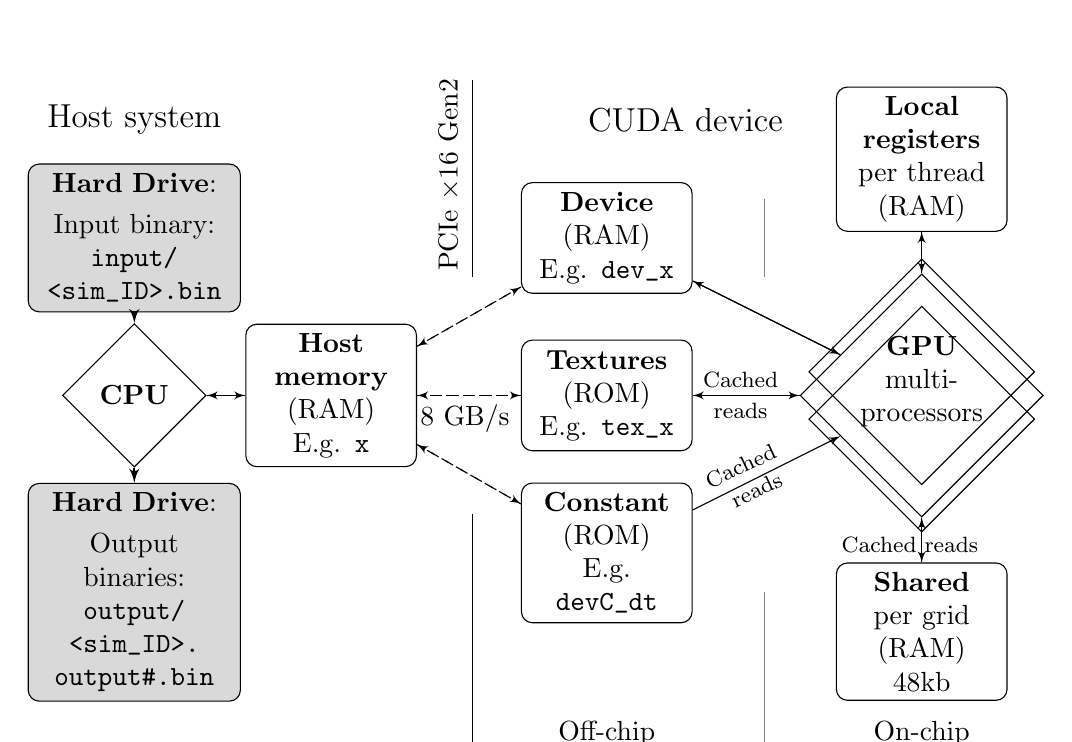
\begin{tikzpicture}[scale=1, node distance = 2cm, auto]
    % Place nodes
    \node [harddrive] (freadbin) {\textbf{Hard Drive}:\\[1mm] Input binary: \verb"input/"\\\verb"<sim_ID>.bin"};
    		
		\node [processor, below of=freadbin, node distance=2cm] (cpu) {\textbf{CPU}};
		
    \node [harddrive, below of=cpu, node distance=2.5cm] (fwritebin) {\textbf{Hard Drive}:\\[1mm] Output binaries: \texttt{output/}\\ \verb"<sim_ID>."\\\verb"output#.bin"};
    
		\node [mem, right of=cpu, node distance=2.5cm] (host) {\textbf{Host memory} (RAM) E.g. \texttt{x}};
		
		\node [mem, right of=host, node distance=3.5cm] (textures) {\textbf{Textures} (ROM)\\ E.g. \verb"tex_x"};
		\node [mem, above of=textures, node distance=2cm] (device) {\textbf{Device} (RAM)\\ E.g. \verb"dev_x"};
		\node [mem, below of=textures, node distance=2cm] (constant) {\textbf{Constant} (ROM)\\ E.g. \verb"devC_dt"};
		
		
		\node [processor, right of=textures, node distance=4cm] (gpu) {\textbf{GPU}\\multi-\\processors\\\vrule width 2.1cm};
		
	
        \draw node [above of=gpu, shape aspect=1, diamond, draw, node distance=0.3cm] {\vrule width 2.4cm};
        \draw node [below of=gpu, shape aspect=1, diamond, draw, node distance=0.3cm] {\vrule width 2.4cm};
        
        \node [mem, above of=gpu, node distance=3cm] (local) {\textbf{Local registers} per thread\\ (RAM)};

    	\node [mem, below of=gpu, node distance=3cm] (shared) {\textbf{Shared} per grid\\ (RAM) 48kb};
    
    % Place hardware description
    \node [above of=freadbin, node distance=1.5cm] {\large Host system};
    %\node [above of=device, node distance=4cm] {\Large CUDA device};
    \node [at={(7.0,1.5)}] {\large CUDA device};
    
    \node [at={(4.0,0.8)}, rotate=90] {PCIe $\times$16 Gen2};
    \path [draw] (4.3, 2.0) -- (4.3,-0.5);
    \path [draw] (4.3,-3.5) -- (4.3,-6.5);
    
    \node [at={(6.0,-6.3)}] {Off-chip};
    
    \path [draw, gray] (8.0, 0.5) -- (8.0,-0.5);
    \path [draw, gray] (8.0,-4.5) -- (8.0,-6.5);
    
    \node [at={(10.0,-6.3)}] {On-chip};
    
    % Draw lines
    \path [draw, -latex', thick] (freadbin) -- (cpu);
    
    \path [draw, -latex'] (cpu) -- (host);
    \path [draw, -latex'] (host) -- (cpu);

    \path [draw, -latex', dashed] (host) -- (device);
    \path [draw, -latex', dashed] (device) -- (host);

    \path [draw, -latex', dashed] (host) -- (constant);
    \path [draw, -latex', dashed] (constant) -- (host);
    %\path [draw, -latex'] (constant) -- (device);
    
    \path [draw, -latex', dashed] (host) -- (textures);
    \path [draw, -latex', dashed] (textures) -- (host);
    
    %\path [draw, -latex', dashed] (host) -- (shared);
    %\path [draw, -latex', dashed] (shared) -- (host);
    
    \path [draw, -latex'] (device) -- (gpu);
    \path [draw, -latex'] (gpu) -- (device);
    
    \path [draw, -latex'] (textures) -- (gpu);
    \path [draw, -latex'] (gpu) -- (textures);
    \node [at={(7.7,-1.8)}] {\footnotesize Cached};
    \node [at={(7.7,-2.2)}] {\footnotesize reads};
    
    \path [draw, -latex'] (constant) -- (gpu);
    %\path [draw, -latex'] (gpu) -- (constant);
    \node [at={(7.7,-2.9)}, rotate=25] {\footnotesize Cached};
    \node [at={(7.9,-3.2)}, rotate=25] {\footnotesize reads};
    
    \path [draw, -latex'] (shared) -- (gpu);
    \path [draw, -latex'] (gpu) -- (shared);
    \node [at={(9.85,-3.9)}] {\footnotesize Cached reads};
    %\node [at={(8.0,-4.2)}, rotate=45] {\footnotesize reads};
    
    \path [draw, -latex'] (local) -- (gpu);
    \path [draw, -latex'] (gpu) -- (local);
    
    
    %\path [draw, -latex'] (device) -- (shared);

    \path [draw, -latex', thick] (cpu) -- (fwritebin);
    
    % Bandwith text
    \node [at={(4.2,-2.3)}] (host-dev) {8 GB/s};
    %\node [at={(3,-3)}] (PCIe)�{(PCIe Gen2)};
    %\node [at={(6,-2.3)}] (dev-dev) {89.6 GB/s};

\end{tikzpicture}
\end{small}

\caption{Flow chart of system memory types and communication paths. RAM: Random-Access Memory (read + write), ROM: Read-Only Memory. Specified communication path bandwidth on test system (2010 Mac Pro w. Quadro 4000 noted.}
\end{center}

\end{figure}


\paragraph{Host memory} is the main random-access computer memory (RAM), i.e. read and write memory accessible by CPU processes, but inaccessible by CUDA kernels executed on the device. 


\paragraph{Device memory} is the main, global device memory. It resides off-chip on the GPU, in the form of up to 2GB DRAM.


\paragraph{Constant memory}


\paragraph{Textures}





\subsection{The main loop}
\label{subsec:mainloop}
The \texttt{SPHERE} software calculates particle movement and rotation based on the forces applied to it, by application of Newton's law of motion (Newton's second law with constant particle mass: $F_{\mathrm{net}} = m�\cdot a_{\mathrm{cm}}$). This is done in a series of algorithmic steps, see list on page \pageref{loopstart}. The steps are explained in the following sections with reference to the \texttt{SPHERE}-source file; \texttt{sphere.cu}. The intent with this document is \emph{not} to give a full theoretical background of the methods, but rather how the software performs the calculations.









\subsection{Performance}
\subsubsection{Particles and computational time}
With an increasing amount of particles, obviously more calculations have to be performed each time step, which directly translates to an increasing computational time. 

The size of the computational timestep length is fixed at a sufficiently low value, so that the particle response is calculated several times while the speed of sound (the strain signal) travels through even the smallest particle, see equation \ref{eq:dt}. If there is a large variety of particle sizes, the particle with the smallest radius determines \texttt{dt} for all calculations.

\subsubsection{Parallel computing}
The \texttt{DISC} code is heavily parallized, i.e. it does carries out multiple calculations simultaneously, utilizing the GPU. 

\subsubsection{Compute profiler results}


\subsection{Compilation}
\label{subsec:compilation}
\texttt{SPHERE} is supplied with a makefile which helps the compilation process. Open a terminal, go to the \texttt{src/} subfolder and type \texttt{make}. The GNU Make will return the parameters passed to the individual CUDA and GNU compilers (\texttt{nvcc} and \texttt{gcc}). The resulting binary file (\texttt{sphere}) is placed in the \texttt{SPHERE} root folder.



\section{Model setup}
\label{sec:ModelSetup}
In {\sc Matlab}, enter the \texttt{mfiles/}-directory as the current folder (example: \texttt{>> cd ~/code/sphere/mfiles/}). For each new experiment setup, it might be a good approach to copy the software root-folder, thus saving past configurations and data.

\subsection{Creating the particles}
To begin with, the model surroundings and the particles are created. Particle sizes are randomly drawn from either a \emph{log-normal}- or \emph{uniform} distribution. These particles are situated in a fixed grid-like setup. 

Using the {\sc Matlab} Editor or another editor, open the file \texttt{mfiles/initsetup.m}. Here you set:
 \begin{itemize}
  \item The filename of the output file (\texttt{fn})
  \item The number of particles (\texttt{p.np})
  \item The particle size distribution (\texttt{logn}: log-normal or \texttt{uni}: uniform), including
    \begin{itemize}
      \item Mean size (\texttt{p.m})
      \item Variance (\texttt{p.v})
    \end{itemize}
  \item Physical parameters (\texttt{params.g}: gravity, \texttt{p.rho}: density, \verb"p.k_n": normal stiffness, \verb"p.k_s": shear stiffness), etc...)
  \item Time parameters (\texttt{time.dt}: computational time step length, \texttt{time.current}: starting time, \texttt{time.total}: total simulation time, \verb"time.file_dt": interval between output generation)
\end{itemize}
After any modifications the file needs to be saved. Write the specified model setup using the following command in {\sc Matlab}:
\begin{lstlisting}
    >> initsetup
\end{lstlisting}
This will write the binary file for \texttt{SPHERE} to read, display a histogram of the particle size distribution, and show a figure of the model setup. 




\subsection{Introducing heterogenieties}
Until now, all grains in the model have the same physical properties. Heterogenieties can be introduced in the same way as the coloring above. The \texttt{find()}-function in {\sc Matlab} can be used to set different properties on particles, that fulfill a specific requirement, e.g. are contained between geometric border-values in the coordinate system in the initial setup.

Please note, that these deviant values need to be set \emph{after} the general physical values in \texttt{template.m}.
The following is an example, that assigns new values for cohesion ($C$) and angle of internal friction ($\phi$) for the bottom 0.02 m particles:
\begin{lstlisting}
    %%Heterogenieties
    %Weak bottom layer
    y = p.x(:,2);
    I = find(y < 0.02); %Particles defined as quantity I
    phi = 1; %Angle of internal friction
    DEM.particles.friction(I) = tan(phi*pi/180)*ones(length(I),1);
    C = 10; %Cohesion
    DEM.particles.cohesion(I) = C*ones(length(I),1);
    DEM.particles.matflag(I) = 2;
\end{lstlisting}
Here, the affected particles are given a different \texttt{matflag}-value, for visual identification of the particles with different properties.

\subsection{Periodic boundary conditions}
\label{subsec:CyclicBorder-conditions}
For simulating mechanisms that involve large horizontal strains, as in a ring-shear apparatus, it is a good approach to make the left and right borders cyclic. That means that a particle disappearing out of the right  side will reappear in the same vertical position in the left side. Particles can affect each other with contact forces in the same way.
This has the advantage that the total number of particles can be kept low in relation to a very wide model setup.

The cyclic borders are in {\sc Matlab} enabled by the command \texttt{DEM.rm.periflag = 1}. In this configuration, only the top and bottom walls are needed. A specific normal-pressure is applied in pascal ($Pa^{-1} = \frac{N}{m}$) (denote the value with a negative sign for downward oriented pressure). The shearing motion is applied by fixing the bottom particles to a horizontal velocity of zero (0), and moving the uppermost particles at a constant horizontal velocity (e.g. $0.1 \frac{m}{s}$). The particles are not fixed in the vertical directions, since particles still need to be able to pass each other by volumetric expansion.
 


\section{DEM simulation using \texttt{SPHERE}}
\label{sec:Simulation}
After the initial model preferences have been set up in {\sc Matlab} and the binary input file is written, the DEM-calculations can be initialized from the terminal. Specify the input file name as a parameter for \texttt{SPHERE}:
\begin{lstlisting}
    $ ./sphere simulation_name
\end{lstlisting}
In {\sc Matlab}, the state of the calculations can be checked with:
\begin{lstlisting}
    >> status('simulation_name')
\end{lstlisting}
The basics of the DEM algorithm, used in \texttt{SPHERE}, is described in section \ref{sec:Theory}, page \pageref{sec:Theory}. While \texttt{SPHERE} is running, output binary files are placed in the \texttt{output/} folder with the format \texttt{simulation\_name.output\#.bin}. On UNIX systems, the CPU usage of active processes can be monitored with the command '\texttt{top}'. GPU usage is monitored using e.g. the NVIDIA Compute Visual Profiler.


\section{Data analysis in {\sc Matlab}}
\label{sec:DataAnalysis}
A number of preconfigured visualization methods are featured in \texttt{show.m}. It shows a figure of the particle assemblage, created on base of the data from a specific output-file. This output file is selected with the command \verb"show('file',#)", where the second parameter is the number of the output file (the numbering starts from zero (0)).  Even though the SDEM calculations (\texttt{./start}-script) have not been completed, the latest output file can be visualized in {\sc Matlab}, as long as at least one output-file has been generated:
\begin{lstlisting}
    >> show('file','latest')
\end{lstlisting}
A series of graphs, including total kinetic energy, dissipation energy, number of particles and time steps as functions of time can be displayed with:
\begin{lstlisting}
    >> show('energy')
\end{lstlisting}
When defining a wall-position as a function of pressure, not velocity, all wall velocities can be displayed with:
\begin{lstlisting}
    >> show('wallspeed')
\end{lstlisting}
And if the wall-position is a function of velocity, not pressure, the wall pressures can be displayed with:
\begin{lstlisting}
    >> show('wallforce')
\end{lstlisting}
The total accumulated horizontal displacement of the particles:
\begin{lstlisting}
    >> show('sheardisp')
\end{lstlisting}
If simulating a shearing motion, it may be desired to create a graph, that shows the horizontal velocity of each particle. This is done by using the \texttt{'veloprofile'}-option in \texttt{show()}, for example:
\begin{lstlisting}
    >> show('file','latest','veloprofile')
\end{lstlisting}
Additional arguments can be used in the \texttt{show}-command, to visualize various parameters, i.e. pressure or strain for each particle. The \texttt{colorbar}-function adds a bar explaining the values and colors:
\begin{lstlisting}
    >> show('file','latest','field','pressure')
    >> colorbar
    >> show('file','latest','field','eplast')
    >> colorbar
\end{lstlisting}
For displaying the colorbar with a fixed span:
\begin{lstlisting}
    >> show('file','latest','field','eplast','clim',[0;5])
    >> colorbar
\end{lstlisting}

\subsection{Exporting plots}
The {\sc Matlab} function \texttt{exportplots(mode)} is included for automatically plotting a range of output files, and exporting them as image files. It plots the raw DEM-data from the last run experiment with show() and saves the output as image files. Open \texttt{mfiles/exportplots.m}, and check the folder, filename and graphics format settings. After saving, call the function in {\sc Matlab}:
\begin{lstlisting}
    >> exportplots()
\end{lstlisting}
This creates an image for each output file in the \texttt{output/} directory, and with the default settings, saves them in the folder \texttt{flic/}. During the process, {\sc Matlab} will display a waitbar, showing the progress. If needed, the export may be halted by clicking the 'Cancel' button in the waitbar window. \underline{Do not} press \texttt{Ctrl-C}; after killing the export this way, a restart of {\sc Matlab} is needed before repeating the command. If, for some reason, the code crashes wile running, the waitbar is forcibly closed by:
\begin{lstlisting}
    >> set(0,'ShowHiddenHandles','on')
    >> delete(get(0,'Children'))
\end{lstlisting}
To export the plots with particles colored according to the elastic plasticity or pressure:
\begin{lstlisting}
    >> exportplots('eplast')
    >> exportplots('pressure')
\end{lstlisting}
To create a plot over the velocity profile for each output file, and exporting it:
\begin{lstlisting}
    >> exportplots('veloprofile')
\end{lstlisting}
To export all normal-, eplast-, pressure and veloprofiles as images use the command \texttt{exportall()}, which creates a series of images (combi) containing the four view modes simultaneously:
\begin{lstlisting}
	>> exportall(1)
\end{lstlisting} 
When the goal of the export is to create an animation in the \texttt{avi} or \texttt{mpeg}-format, I recommend exporting to the \texttt{jpeg}-format, which can be chosen in \texttt{exportplots.m}. In most video editing software the \texttt{png}-format is only poorly, if at all, supported.

\subsection{Importing data}
All parameters and values from the simulation results can be imported into the {\sc Matlab} workspace. In {\sc Matlab}, make sure the current folder is the \texttt{mfiles/} directory inside the \texttt{DISC} folder. The DEM structure from the current configuration is loaded by \texttt{DEM = DEMload()}, which reads \texttt{input/DEM.mat}. The resulting variable structure imported into the {\sc Matlab} workspace, and consists of a hierarchy of variables, as mapped out in appendix \ref{apx:DEMParameterStructureInMatlab}. 
While \texttt{DEMload()} loads the initial model setup, the {\sc Matlab} function \texttt{DEMloadfnr(fnr)} loads particle configurations from output file with number \texttt{fnr}. 

The following is a number of examples, showing possible ways to visualize particle speed\footnote{Inspired by: \url{http://geology.wlu.edu/connors/primers/Surfaces_and_Grids_in_Matlab/Surfaces_and_Grids_in_Matlab.htm}}. The following series of commands loads all particle positions and creates a three-dimensional plot with speed on the z-axis from output file \#25:
\begin{lstlisting}  
	>> [p, grid, time, params] = freadbin('../output/', 5);
	>> x=p.x(:,1);
	>> y=p.x(:,2);
	>> z=sqrt(p.vel(:,1).^2+p.vel(:,2).^2);
	>> plot3(x,y,z,'.')
\end{lstlisting}
Or as a triangular surface for better visualization; lone points distributed in a 3D space, visualized in 2D, are difficult to comprehend visually:
\begin{lstlisting}
	>> tri=delaunay(x,y);
	>> trisurf(tri,x,y,z)
\end{lstlisting}
Or as a (smoothed) surface with interpolated data point values in between particles:
\begin{lstlisting}
	>> res=100; %Resolution in x- and y-direction
	>> rangeX=min(x):(max(x)-min(x))/res:max(x);
	>> rangeY=min(y):(max(y)-min(y))/res:max(y);
	>> [X,Y]=meshgrid(rangeX,rangeY);
	>> Z=griddata(x,y,z,X,Y);
	>> surf(X,Y,Z)
\end{lstlisting}
To make a contour plot of the gridded data:
\begin{lstlisting}
	>> resZ=100; %Resolution in z-direction
	>> rangeZ=min(z):(max(z)-min(z))/resZ:max(z);
	>> contourf(X,Y,Z,rangeZ);
\end{lstlisting}
Combining contours and surfaces:
\begin{lstlisting}
	>> hold on
	>> surf(X,Y,Z,'EdgeColor','none','FaceColor','interp','FaceLighting','phong')
	>> contour3(X,Y,Z,rangeZ,'k')
	>> figure(gcf)
\end{lstlisting}
Another example: Arrow field of particle velocities:
\begin{lstlisting}
	>> s=0.02; %Velocity scaling factor
	>> quiver(p.x(:,1), p.x(:,2),...
	   p.vel(:,1)*s, p.vel(:,2)*s,'AutoScale','off');
	>> axis([0 0.2 0 0.11])
\end{lstlisting}







\newpage
\appendix
\section*{Appendix}
\section{Folder structure}
\label{apx:FolderStructure}
\texttt{SPHERE} sub directory and file description:

{ \small
\begin{itemize}
  %\item '\texttt{configs/}': Folder for initial particle configurations (\texttt{.mat}-files)
  \item '\texttt{cudaprofiler/}': Folder for saving CUDA Compute Visual Profiler project data.
  \item '\texttt{doc/}': Folder containing documentation
    \begin{itemize}
      \item '\texttt{graphics/}': Documentation image files
  	  \item '\texttt{sphere-doc.pdf}': This document
	  \item '\texttt{sphere-doc.tex}': \LaTeX{} source code for this document
	  \item Auxillary \LaTeX{} files
	\end{itemize}
  \item '\texttt{flic/}': Folder for image creation plugins (not included)
    \begin{itemize}
  	  \item '\texttt{eps/}': EPS image format directory
  	  \item '\texttt{gif/}': GIF image format directory
  	  \item '\texttt{png/}': PNG image format directory
    \end{itemize}
  \item '\texttt{include/}': Directory for preprocessor-files, utilized in \texttt{sphere.cu}.
    \begin{itemize}
  	  \item '\texttt{nrutil.h}': Numerical recipes header file.
	  \item '\texttt{random.c}': Contains the function ran0(...) that returns a random number.
    \end{itemize}
  \item '\texttt{input/}': Folder for simulation configuration binaries.
  \item '\texttt{mfiles/}': Files which contain functions available to {\sc Matlab}.
    \begin{itemize}
      \item '\texttt{bubbleplot.m}': \texttt{bubbleplot(p)} plots particles in structure \texttt{p} using \texttt{bubbleplot3.m}
      \item '\texttt{bubbleplot3.m}': \texttt{bubbleplot(x,y,z,r)} Produces a three-dimensional bubble plot of spheres with coordinates (x,y,z) and radius (r). Created by Peter Bodin, obtained through Mathworks File Exchange\footnote{\url{http://www.mathworks.com/matlabcentral/fileexchange/8231-bubbleplot3}}.
      \item '\texttt{freadbin.m}': \texttt{[p, grid, time, params] = freadbin(path, fn)} reads binary file named \texttt{fn} in directory \texttt{path}, and returns {\sc Matlab} structures (appendix \ref{apx:DEMParameterStructureInMatlab}).
      \item '\texttt{fwritebin.m}': \texttt{fwritebin(path, fn, p, grid, time, params)} writes {\sc Matlab} structures (appendix \ref{apx:DEMParameterStructureInMatlab}) to binary file named \texttt{fn} in directory \texttt{path}.
  	  \item '\texttt{initsetup.m}': \texttt{initsetup()} creates particles in grid-like arrangement. The number of particles and the PSD is specified. Calling the function creates a \texttt{.bin}-file in the \texttt{input/}-folder.
      \item '\texttt{status.m}': \texttt{status('simulation\_name')} writes the status of the current model run to the command window.
    \end{itemize}

  \item '\texttt{output/}': Folder containing output \texttt{.bin}-files.   For each output time-step (\texttt{time.file\_dt}), a new \texttt{simulation\_name.output\#.bin} is created, where \verb"#" is the output time step number. Simultaneously, the status-file is updated.
  
  \begin{itemize}
  \item '\texttt{simulation\_name.logfile.txt}': Text file containing eventual error messages from the computation.
  \item '\texttt{simulation\_name.output\#.bin}': Main \texttt{SPHERE} output data.
  \item '\texttt{simulation\_name.status.dat}': File showing the completed calculation progress in percentage, and time steps.
  \end{itemize}

  
  \item '\texttt{src/}': Folder containing \texttt{SPHERE} source code.
  
\end{itemize}
} %end small

\newpage
\section{\texttt{SPHERE} source code variables}
\label{apx:SourceCodeVariables}
Variables without a prefix are located in the host memory. Variables with the prefix '\texttt{dev\_}' are stored in the read \& write device memory, '\texttt{tex\_}' means data is stored in the read-only texture memory on the device.

\begin{table}[hb]
  \centering 
  {\small
  \begin{tabularx}{1.0\textwidth}{p{3cm} l X}
  \textbf{Name} & \textbf{Type} & \textbf{Description}\\
\hline
\texttt{x[i]\{.x,.y,.z\}} \texttt{dev\_x[i]\{.x,.y,.z\}} \texttt{tex\_x[i]\{.x,.y,.z\}} & float4 & Particle coordinates. Returns the coordinates of particle \texttt{i}, optionally only the value in dimension x, y or z. E.g. \texttt{x[124].x} returns x-axis placement of particle 124, read from host memory. \\

\hline
\end{tabularx}
	}%End font size
  \caption{Some important variables in \texttt{sphere.cu}. The integer \texttt{i} refers to the particle number. Curly brackets (\{\}) indicate optional, exclusive extensions.}
  \label{tab:vars}
\end{table}


\newpage
\section{Parameter structure in {\sc Matlab}}
\label{apx:DEMParameterStructureInMatlab}
The DEM structure from the current configuration is loaded into {\sc Matlab} by the command \texttt{[p, grid, time, params] = freadbin(path, fn)}, which reads the specified binary file. The resulting variable structures imported into the {\sc Matlab} workspace are the following:

\vspace{1cm}

%\vfill



\begin{table}[hb]
  \centering 
{\small

%\begin{table}[htb]
%  \centering 
  \begin{tabularx}{1.0\textwidth}{l l X}
\texttt{p.}      & \texttt{np}          & Number of particles\\
        ~        & \texttt{psd}         & Particle size distribution\\
        ~        & \texttt{m}           & Mean particle radius\\
        ~        & \texttt{v}           & Particle radius variance\\
        ~        & \texttt{radius}      & Radius of all particles\\
        ~        & \texttt{x}           & Particle positions in $E^3$ (x,y,z)\\
        ~        & \texttt{vel}         & Particle linear velocities\\
        ~        & \texttt{angvel}      & Particle angular velocities\\
        ~        & \texttt{vel0}        & Fixed linear particle velocitis\\
        ~        & \texttt{force}       & Sum of forces upon each particle\\
        ~        & \texttt{torque}      & Sum of torque upon each particle\\
        ~        & \texttt{rho}         & Particle material densities\\
        ~        & \texttt{k\_n}        & Particle normal stiffnesses\\
        ~        & \texttt{k\_s}        & Particle shear stiffnesses\\
        ~        & \texttt{mu}          & Inter-particle contact friction coefficients\\
        ~        & \texttt{C}           & Inter-particle tensile strengths (cohesion)\\
        ~        & \texttt{E}           & Young's modulus for each particle\\
        ~        & \texttt{K}           & Bulk modulus for each particle\\
        ~        & \texttt{nu}          & Poisson's ratio for each particle\\
\texttt{time.}   & \texttt{dt}          & Computational time step length\\
        ~        & \texttt{current}     & Current time\\
        ~        & \texttt{total}       & Total simulation time\\
        ~        & \texttt{file\_dt}    & Interval between output file generation\\
        ~        & \texttt{step\_count} & Current step count\\
\texttt{grid.}   & \texttt{nd}          & Number of dimensions\\
        ~        & \texttt{origo}       & Cartesian space origo\\
        ~        & \texttt{num}         & Number of grid cells in each dimension\\
        ~        & \texttt{L}           & Grid length in each dimension\\
\texttt{params.} & \texttt{g}           & Gravitational acceleration\\
        ~        & \texttt{global}      & Equals 1: Particle mechanical parameters are global, equals 0: Particle mechanical parameters are individual and set in the \texttt{p} structure.
  \end{tabularx}
	}%End font size
  \caption{{\sc Matlab} variable structure}
  \label{tab:Matlabvars}
\end{table}
\noindent The values are written using the corresponding command \texttt{fwritebin(path, fn, p, grid, time, params)}. 


\newpage
\section{Sample: initsetup.m }
\label{apx:TemplateShear}
\begin{lstlisting}[frame=single,numbers=left,language=MATLAB,basicstyle=\footnotesize]
 function initsetup()
% initsetup() creates a model setup of particles in 3D with cubic
% packing. Specify PSD and desired number of particles, and the 
% function will determine the model dimensions, and fill the space 
% with a number of particles from a specified particle size distribution.
close all;

%Simulation project name
simulation_name = '3dtest';

%Physical, constant parameters
params.g = 9.80665; %standard gravity, by definition 9.80665 m/s^2

% No. of dimensions
grid.nd = 3;
grid.origo = [0 0 0]; %Coordinate system origo

% Number of particles
p.np = 5e2; 

% Create grid
grid.num = ceil(nthroot(p.np,grid.nd)) * ones(grid.nd, 1); %Square/cubic
p.np = grid.num(1)^grid.nd;

%% Particle size distribution
p.psd = 'logn'; %PSD: logn or uni

p.m = 440e-6; %Mean size
p.v = p.m*0.00001; %Variance
%p.m = 22; %Mean size
%p.v = p.m*0.001; %Variance

p.radius = zeros(1, p.np);
p.x      = zeros(p.np, grid.nd);

if strcmp(p.psd,'logn') %Log-normal PSD. Note: Keep variance small.
    mu = log((p.m^2)/sqrt(p.v+p.m^2));
    sigma = sqrt(log(p.v/(p.m^2)+1));
    p.radius = lognrnd(mu,sigma,1,p.np); %Array of particle radii 
elseif strcmp(p.psd,'uni') %Uniform PSD between rmin and rmax
    rmin = p.m - p.v*1e5;
    rmax = p.m + p.v*1e5;
    %rmin = 0.1*dd; rmax = 0.4*dd;
    p.radius = (rmax-rmin)*rand(p.np,1)+rmin; %Array of particle radii
end

%%Display PSD
figure(2);hist(p.radius);
title(['PSD: ' num2str(p.np) ' particles, m = ' num2str(p.m) ' m']); 


%% Other particle parameters
p.vel    = zeros(p.np, grid.nd); % Velocity vector
p.angvel = zeros(p.np, grid.nd); % Angular velocity
p.vel0   = zeros(p.np, grid.nd); % Pre-velocity vector
p.force  = zeros(p.np, grid.nd); % Force vector
p.torque = zeros(p.np, grid.nd); % Torque vector

params.global = 1; % 1: Physical parameters global, 0: individual per particle
p.rho   = 3600*ones(p.np,1);    % Density
p.k_n   = 109680*ones(p.np,1);  % Normal stiffness
p.k_s   = 109680*ones(p.np,1);  % Shear stifness
p.mu    = 1*ones(p.np,1);       % Inter-particle contact friction coefficient
p.C     = 0*zeros(p.np,1);      % Inter-particle cohesion
p.E     = 10e9*ones(p.np,1);    % Young's modulus
p.K     = 38e9*ones(p.np,1);    % Bulk modulus
p.nu    = 0.38*ones(p.np,1);    % Poisson's ratio

%Time parameters
time.dt         = 1e3*0.5*min(sqrt((p.rho(:).*p.radius(:).^2)./p.K(:))); %Computational delta t
time.current    = 0.0;
time.total      = 1.0; %Total simulation time [s]
time.file_dt    = 0.1; %Interval between output#.bin generation [s]
time.step_count = 0;

%% Calculate particle coordinates
%Grid unit length. Maximum particle diameter determines grid size
GU = 2*max(p.radius)*1.10; % Ten percent margin
%Model world side length (cubic arrangement)
grid.L = [GU*grid.num(1) GU*grid.num(2) GU*grid.num(3)];

%% Particle coordinates by filling grid.
x = GU/2:GU:grid.L(1);
y = GU/2:GU:grid.L(2);
z = GU/2:GU:grid.L(3);

% Wall coordinates
 walls = [0,0,0         , grid.L(1),0,0         , grid.L(1),0,grid.L(3)         , 0,0,grid.L(3)         ; ... %Bottom wall (x,z plane)
          0,grid.L(2),0 , grid.L(1),grid.L(2),0 , grid.L(1),grid.L(2),grid.L(3) , 0,grid.L(2),grid.L(3) ; ... %Top wall (x,z plane)
          0,0,0         , 0,grid.L(2),0         , grid.L(1),grid.L(2),0         , grid.L(1),0,0         ; ... %Front wall (x,y plane)
          0,0,grid.L(3) , 0,grid.L(2),grid.L(3) , grid.L(1),grid.L(2),grid.L(3) , grid.L(1),0,grid.L(3) ; ... %Back wall (x,y plane)
          0,0,0         , 0,grid.L(2),0         , 0,grid.L(2),grid.L(3)         , 0,0,grid.L(3)         ; ... %Left wall (y,z plane)
          grid.L(1),0,0 , grid.L(1),grid.L(2),0 , grid.L(1),grid.L(2),grid.L(3) , grid.L(1),0,grid.L(3)];     %Right wall (y,z plane)

%% Plot
figure(1);

% %draw walls
    for i=1:6,
      line(walls(i,[1,4]),walls(i,[2,5]),walls(i,[3,6]),'linewidth',2,'color','k');
      line(walls(i,[7,10]),walls(i,[8,11]),walls(i,[9,12]),'linewidth',2,'color','k');
      line(walls(i,[4,7]),walls(i,[5,8]),walls(i,[6,9]),'linewidth',2,'color','k');
      line(walls(i,[10,1]),walls(i,[11,2]),walls(i,[12,3]),'linewidth',2,'color','k');
    end;

[X Y Z] = meshgrid(x,y,z);
X=X(:); Y=Y(:); Z=Z(:);

p.x = [X Y Z]; 

%Particle positions randomly modified by +/- 5 percent
p.x = p.x .* (rand(p.np, grid.nd)*0.1 + 0.95);

%% Plot particles in bubble plot
bubbleplot(p);

%% Write output binary
fwritebin('../input/', [simulation_name '.bin'], p, grid, time, params);

end
\end{lstlisting}

\newpage
\addcontentsline{toc}{section}{References}
\label{sec:References}
\bibliographystyle{plainnat}
\bibliography{/Users/anders/Documents/University/BIB}

\vfill
\begin{center}\small{--- End of file ---}\end{center}
\end{document}
